This chapter presents a general background to the concepts and methods used in the project and reviews the literature related to the problem this project is trying to solve. The first section discusses image feature representation and its evolution, followed by a summary of neural networks, an overview of image processing in deep learning using convolutional neural networks, and ideas of transfer learning and metric learning. The last section presents the previous work on finding similar artworks using visual features.

\section{Image Representation: Hand-Engineered to Learned Features}

An image, seen through human eyes, can be an ensemble of various elements such as landscape, animals, people, text, tools, or any object with shape and form. However, this is not the case with computers, where an image is an array of pixels in Red, Green, and Blue channels. Although the same arrangement of pixels in the image enables humans to interpret the elements, it is not sufficient for computer vision tasks. Thus the \textit{features} that can convey the information present in the image are used to represent it in computer vision tasks. 

Earlier methods involved crafting problem-specific features. Some known handcrafted features useful in object detection and localization include simple histograms and \emph{Histograms of Oriented Gradients} (HOG) \cite{Dalal2005HistogramsOO}. The \emph{Scale-invariant Feature Transform} (SIFT) \cite{lowe2004distinctive} or \emph{Speeded-Up-RobustFeature} (SURF) \cite{BAY2008346} features based on local descriptors are beneficial in comparing images. Artificial neural networks (described in the next section) can benefit from these features. However, this feature engineering step requires expert knowledge.

More often than not, these feature descriptions are based on only one property (like texture, edge, or color) and sensitive to minor variations, and generalize poorly. Convolutional neural networks address this problem of feature engineering where the \textit{convolution} layers transform the input (image) before passing through a feed-forward network to perform classification, detection, or localization. These convolutional layers \textit{learn} the \textit{features} of the image and eliminate the need to hand-engineer them.

\section{Artificial Neural Networks}

\emph{Artificial Neural Networks} (ANN), inspired by the neuron connections in the brain, were ideas proposed nearly seven decades ago. With the increasing computing power and algorithms to train, they have been an active research topic since the 1980s \cite{goodfellow2016deep}. An ANN is composed of layers of neurons, the first layer accepts the inputs and transforms them non-linearly in the hidden (or middle) layers, and the last layer provides the output. The number of neurons in the first and last layers is the number of input and output features of the problem, respectively. The number of hidden layers and the neurons in each layer are hyperparameters. Each neuron accepts the input from all the neurons in the previous layer, multiplies it by a certain weight, and transforms it using non-linear functions such as Sigmoid, TanH, or ReLU. If there are no hidden layers, an ANN is a non-linear function applied to the input, and adding multiple hidden layers makes it a Deep Neural Net. The weights between the layers are initialized randomly and optimized until the network meets the desired criteria. The networks are commonly optimized using the backpropagation algorithm that propagates the error from the output to the input layer and updates the weights using gradient descent methods. 

Input to an ANN is one dimension vector and thus makes it difficult to process images that are three-dimensional tensors with Height, Width, and Color (usually three) dimensions. Although it is possible to flatten a three-dimensional image into a one-dimensional vector, it increases the size of the network. Hence, the images are represented using a handcrafted feature vector and presented as an input to the ANN. The previous section mentions the drawbacks of using hand-engineered features, and Convolutional Neural Networks are used to overcome them.

\section{Convolutional Neural Networks}

\emph{Convolutional Neural Networks} (CNN) accept the image tensor in its original form and passes it through convolutional layers before flattening and passing it through a fully connected layer to perform classification or prediction. The operation in the convolutional layers is similar to the conventional image processing convolution operation. However, the weights of filters are not predetermined but updated when training the network to perform the desired task. Although a tensor of any shape can be an input to the CNNs, as they primarily process images, the rest of the thesis assumes an image as an input to the convolutional network.

\begin{figure}[ht]
\centering
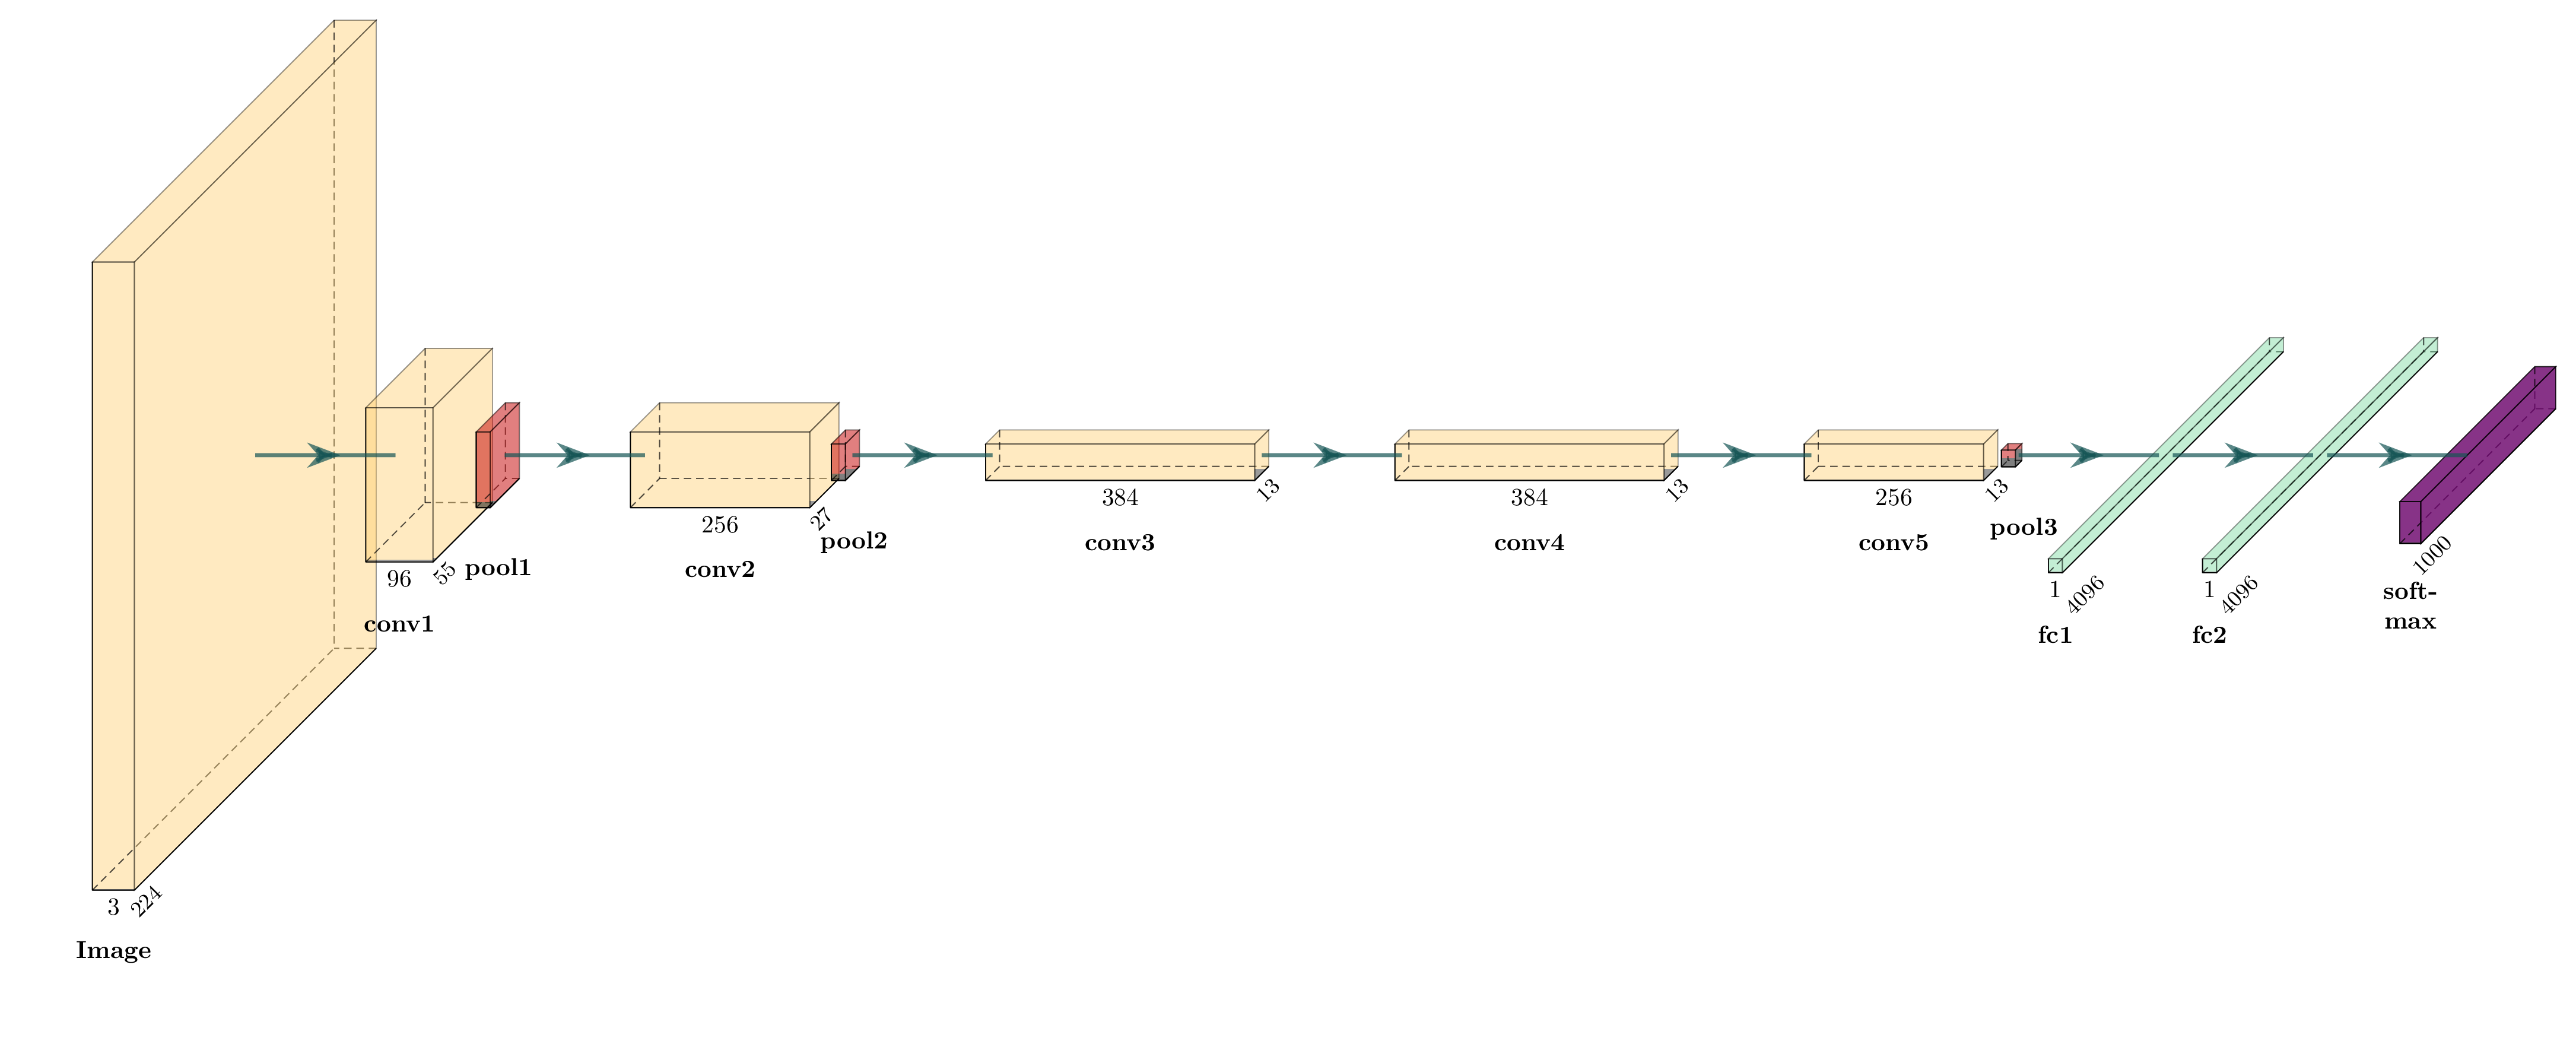
\includegraphics[width=\textwidth]{images/alexnet/alexnet.png}
  \caption{Alexnet \cite{krizhevsky2012imagenet} architecture, revisualized using \cite{haris_iqbal_2018_2526396}}
  \label{fig:alex-net}
\end{figure}

The \textit{Alexnet} \cite{krizhevsky2012imagenet} proposed in 2012 brought back the attention to CNNs when it used Graphics Processing Units to train the model and won the \textit{ImageNet Large Scale Visual Recognition Challenge} \cite{russakovsky2015ILSVRC} by a margin of nearly eleven percentage points compared to the next best performance. \textit{Alexnet} (Figure \ref{fig:alex-net}) has five convolutional layers (prefix \textit{conv}), and in between them, pooling layers, indicated with prefix \textit{pool}, are used to reduce the dimension of the output. The output of the last convolutional layer is flattened and passed through two fully connected layers (prefix \textit{fc}) before predicting the class of the image (out of 1000 possible classes) in the last layer. Thus, the intermediate convolutional layers on the CNN \textit{learn} hierarchal features while solving the problem, and the convolutional layers act as feature extractors.

\subsection{Residual Networks}

After \textit{Alexnet}, many variations of the CNNs - Residual, Inception, Dense, Highway, Attention-based networks, and various learning tricks - Data Augmentation, Dropout, Rectified Linear Unit activation, Batch Normalization came into existence. Out of such improvements, residual networks proposed by Kaiming et al. \cite{He2016DeepRL} became popular to fight the problem of \textit{vanishing gradients} in deep networks. During multi-layered neural network training, the gradient (change in weight with respect to the error) used to modify the weight becomes negligible (vanishes) before updating the initial layers because of the depth. The residual networks try to solve this problem by using a skip connection that adds a link between two points in a network to skip any modification on the input. Figure \ref{fig:resnet} shows a residual block (presented in \cite{He2016DeepRL}). This technique retains the original properties of the input image and the already learned transformations on it.

\begin{figure}[ht]
\centering
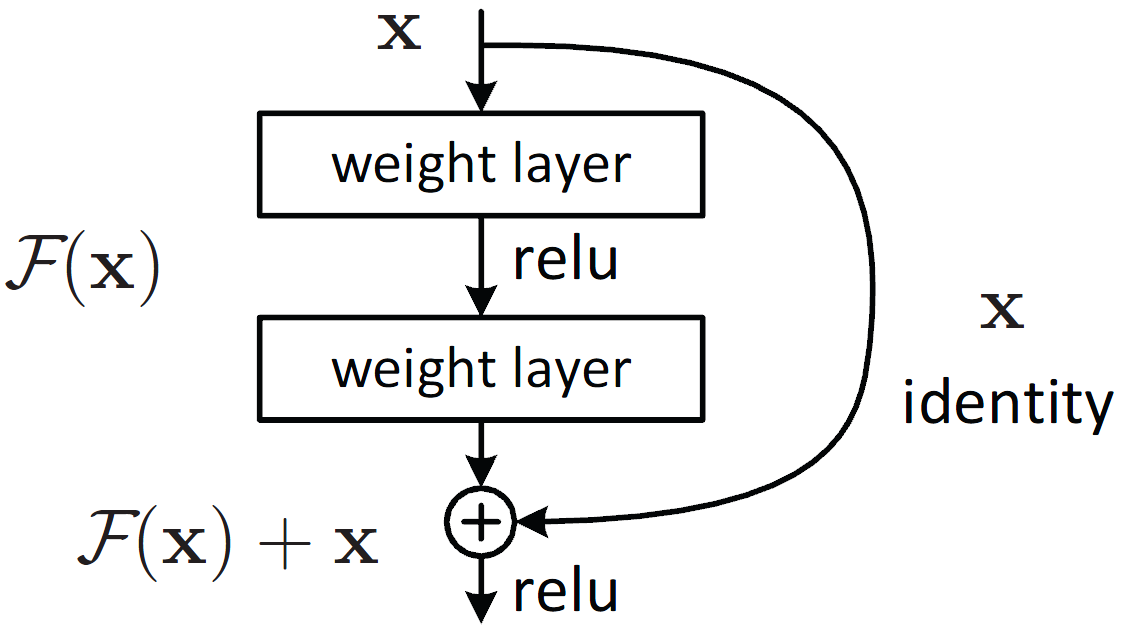
\includegraphics[width=0.6\textwidth]{images/resnet/resnet.png}
  \caption{Residual block with a skip connection. Adapted from \cite{He2016DeepRL}.}
  \label{fig:resnet}
\end{figure}

\subsubsection{ResNeXt}

Another family of CNNs are Inception models that use a split-transform-merge strategy. The inception network splits the input into a few lower dimensional embeddings, transforms them with specialized filters for each embedding (called path), and concatenates through depth to merge them. Although Inception modules are known to have lower computational complexity, their adaption for new tasks/datasets is not clearly defined \cite{Xie2016}. ResNeXt network architecture proposed by Xie et al. \cite{Xie2016} combines the split strategy of the Inception network and the idea of depth from ResNet \cite{He2016DeepRL} that merges the transformed low dimensional inputs by summation instead of concatenation. Additionally, transformations applied to each input embedding are the same. As this architecture is more easily adaptable to new tasks than the Inception networks \cite{Xie2016}, the current project uses a model based on residual connections, specifically the ResNeXt architectures.

\section{Few-shot learning}

The availability of large datasets plays a central role in the success of Deep Learning methods, including other factors like network architecture, learning techniques, and graphic card computation. However, the possibility of obtaining hundreds or thousands of samples to train a neural net is not always high. \emph{Few-Shot Learning} (FSL) approaches are used in training (fine-tuning) classification models when data is scarce. One-shot learning is a sub-category of few-shot learning methods where only one example is available per class. One-shot learning is widely used in computer vision tasks and gained popularity with face recognition studies \cite{koch2015siamese}. Wang et al. \cite{Wang2020FSL} divide FSL methods into three categories. Based on the prior knowledge of the dataset, the first category deals with augmenting the training data, the constraints on the model hypothesis space fall in the second category, and algorithms to provide good initialization or instruct the parameter update. 

The current work also suffers from the problem of fewer examples per class as a drawing generally refers to only one artwork, and all three types of methods mentioned earlier are employed to circumvent it. First, increasing the drawings made by the children by augmenting them into various styles like watercolors, pencil sketches, and oil paintings. Second, utilizing the Task-Invariant Embedding model (Metric Learning through Triplets) and the same model to process drawings and paintings (enables parameter sharing). Lastly, initializing the parameters of the CNN model obtained in training it for a classification task with Imagenet data \cite{deng2009imagenet} and fine-tune it from there (Transfer Learning).

\subsection{Transfer Learning}

Transfer Learning refers to using models trained for one task either for a second task or as a starting point to fine-tune the model for the second task. Generally, transfer learning uses the state of the art models, and the motivation for that is two-fold; training state-of-the-art models use large datasets and heavy computational power, and deep neural nets, especially CNNs, are known to learn the generic features in the convolutional layers \cite{zeiler2014visualizing}. 

There are two most common ways of using CNNs in transfer learning. First, CNNs act as feature extractors to obtain the feature representation of the new images through the convolutional layers of the pre-trained network. These features are then used in conjunction with other Machine Learning algorithms to compare, classify or visualize the data. Many works utilizing the CNNs trained on the ImageNet dataset \cite{deng2009imagenet} have achieved satisfactory performances even when the domain of images is different from the ImageNet \cite{long2015fully, shin2016deep, Schroff2015FaceNetAU}. The second way uses the pre-trained CNN as a starting point, and the network is fine-tuned on the specific dataset instead of end-to-end training the CNN for the new problem. The complexity of the problem and the similarity between the new dataset and the pre-trained CNN dataset determines the layers to retrain.


\subsection{Metric Learning}\label{chap:2:metric-learn}

Clustering, classification, or retrieval of images requires transforming them from their original space into a latent space that uses the feature representation and operations on these feature vectors fulfill the required tasks. Examples include using the euclidean distance between the feature vectors in K-means clustering of images or transforming them into a lower dimension (than the feature vector) space using Principal Component Analysis. However, the distances do not directly affect the creation of the feature vectors. Besides, unlike the classification or regression problems, it is hard to quantify the similarity between images, but it is possible to rank them based on their similarity. The idea of Metric Learning is to use image similarity or dissimilarity directly in training a feature generation model. Metric learning tries to reduce the distance between similar samples and increase the distance between dissimilar ones. Lu et al. \cite{Lu2017DeepML} provide an overview of using metric learning in deep neural nets for vision-related tasks.

% \subsubsection{Siamese networks}

% Siamese networks and triplet networks are the popular variants of neural networks that use metric learning. The former network requires pairs of positive (similar)and negative (dissimilar) samples for training and minimizes a contrastive loss as described in Equation \ref{contrastive_loss} \cite{Lu2017DeepML}.
% If \begin{math} P \end{math} is the set of positive pairs, \begin{math} N \end{math} is the set of Negative Pairs, \begin{math} dist \end{math} computes the distance between two samples \begin{math} i \end{math} and \begin{math} j \end{math}, \begin{math} h(x) = max(0, x) \end{math} is the hinge loss with \begin{math} \tau_{1} \end{math} and \begin{math} \tau_{2} \end{math} being positive threshold that makes the constraint valid with a margin, the contrastive loss is defined as 
% \begin{equation}\label{contrastive_loss}
% L = \sum_{(i, j)\epsilon P}^{} h(dist(\pmb{x}_{i}, \pmb{x}_{j}) - \tau_{1}) + \sum_{(i, j)\epsilon N}^{} h(\tau_{2} - dist(\pmb{x}_{i}, \pmb{x}_{j}))
% \end{equation}
% where \begin{math} \pmb{x}_{n} \end{math} is the feature vector of sample \begin{math} n \end{math}. Minimizing the contrastive loss tries reduce the distance between a positive pair to less than \begin{math} \tau_{1} \end{math} and increase the distance between a negative pair to greater than \begin{math} \tau_{2} \end{math}, where \begin{math} \tau_{2} \end{math} > \begin{math} \tau_{1} \end{math}.


% \subsubsection{Triplet Networks}

% \subsection*{TODO:}
% \begin{enumerate}
%     \item Add image visualizing the triplet learning (borrowed image)
% \end{enumerate}


% The siamese network accepts only positive or negative pairs at a time, and the training might not converge, or the network could overfit the training data. Triplet networks attempt to overcome this shortcoming, and as implied in the name, the network requires three images instead of two at a time for the training \cite{Schroff2015FaceNetAU}. A triplet is composed of an anchor image, a positive sample similar to the anchor image, and a negative one dissimilar to the anchor image. Due to the triplets, the network simultaneously tries to minimize the distance with the positive sample while increasing it with the negative instance, as visualized in Figure \textbf{add figure from the original paper}. For a set \begin{math} T \end{math} of triplets, the triplet network minimizes the triplet loss \cite{Lu2017DeepML} defined as 
% \begin{equation}\label{triplet_loss}
% L = \sum_{(a, p, n) \epsilon T}^{}h(\tau + dist(\pmb{x}_{a}, \pmb{x}_{p}) - dist(\pmb{x}_{a}, \pmb{x}_{n}))
% \end{equation} 
% where \begin{math} \pmb{x}_{a}, \pmb{x}_{p} \end{math} and \begin{math} \pmb{x}_{n} \end{math} are the feature vectors of the anchor, positive and negative samples respectively, \begin{math} dist(\pmb{x}_{a}, \pmb{x}_{p}) \end{math} is the distance between anchor and the positive sample, \begin{math} dist(\pmb{x}_{a}, \pmb{x}_{n}) \end{math} is the distance between anchor and the negative sample, and \begin{math} \tau \end{math} is a positive threshold that makes the constraint valid with a margin or in other words the minimum distance between the positive and the negative samples is \begin{math} \tau \end{math}. 

% Following the testing of two kinds of networks, this work uses the triplet network as its performance was better than the siamese network.


\subsection{Triplet Networks}

Siamese and triplet networks are the popular variants of neural networks that use metric learning. The former network requires pairs of positive (similar) and negative (dissimilar) samples for training and it minimizes a contrastive loss. The siamese network accepts only positive or negative pairs at a time, and the training might not converge, or the network could overfit the training data. Triplet networks attempt to overcome this shortcoming, and as implied in the name, the network requires three images instead of two at a time for the training \cite{Schroff2015FaceNetAU}. A triplet is composed of an anchor image, a positive sample similar to the anchor image, and a negative one dissimilar to the anchor image. Due to the triplets, the network simultaneously tries to minimize the distance with the positive sample while increasing it with the negative instance. For a set \begin{math} T \end{math} of triplets, the triplet network minimizes the triplet loss \cite{Lu2017DeepML} defined as 
\begin{equation}\label{triplet_loss}
L = \sum_{(an, p, n) \epsilon T}^{}h(\tau + dist(\pmb{x}_{an}, \pmb{x}_{p}) - dist(\pmb{x}_{an}, \pmb{x}_{n}))
\end{equation} 
where \begin{math} \pmb{x}_{an}, \pmb{x}_{p} \end{math} and \begin{math} \pmb{x}_{n} \end{math} are the feature vectors of the anchor, positive and negative samples respectively, \begin{math} dist(\pmb{x}_{an}, \pmb{x}_{p}) \end{math} is the distance between anchor and the positive sample, \begin{math} dist(\pmb{x}_{an}, \pmb{x}_{n}) \end{math} is the distance between anchor and the negative sample, and \begin{math} h(x) = max(0, x) \end{math} is the hinge loss with \begin{math} \tau \end{math} as a positive threshold that makes the constraint valid with a margin or in other words the minimum distance between the positive and the negative samples is \begin{math} \tau \end{math}.

\subsubsection{Mining of Triplets}

The selection of positive and negative samples is crucial to ensure convergence of the model training process. The choice for positive examples is straightforward but not easy to get as it requires manual annotation. On the other hand, it is easy to obtain negative samples (all the non-positive instances can be negative samples). However, they could lead to overfitting as their number is far greater than the positives, and at the same time, selecting the negatives that are already far from the anchor will disallow learning in the network. References \cite{Schroff2015FaceNetAU, SimoSerra2015DiscriminativeLO} suggest a hard sampling strategy to counter the under and over fitting, where non-positive artworks proximate to the anchor, obtained using the distance function \begin{math} dist \end{math}, act as negatives in the triplets.

Using metric learning in training a network implies optimizing the distance measure for the task that uses the specific metric. Therefore, using the triplets chosen at the start of the training (offline selection) for the entirety of the training poses an issue where the model could fit triplets, and the loss vanishes, effectively stopping the training. The online triplet selection process deals with this problem, by selecting a new set of triplets after updating the model in each round of training \cite{Schroff2015FaceNetAU}. This work uses the online method of triplet selection.

\section{Related work}\label{chap:2:related_work}

Literature, methods, and engineering techniques related to image retrieval are abundant. This section does not provide a survey of those works but discusses the relevant ones in developing the solutions to the current task.

\subsection{Image Retrieval using Computer Vision}

Following the digital camera revolution and the recent digitization, massive databases of images are a reality. Browsing and searching through these images apiece is difficult even if they are indexed based on name, creation date, or other structural metadata, as people usually wish to explore the databases based on their content. The text queries that operate on the descriptive metadata such as titles, tags of contents, and other image-related keywords aid up to some extent. However, some elements of an image, like its morphological characteristics, cannot be described in words. \emph{Content-Based Image Retrieval} (CBIR) tries to overcome these shortcomings using the visual image contents (color, shape, texture, spatial arrangement).

CBIR systems using the traditional features like GIST, affine-invariant Hessian regions, and SIFT/SURF \cite{Philbin2007ObjectRW} and learned features using CNNs as image descriptors \cite{wan2014deep} are popularly known. As examined by Zhou et al. \cite{Zhou2017RecentAI}, the datasets used in the experiments are photos of landmarks (\textit{Holidays, Paris}), buildings (\textit{Oxford-5K, ZuBuD dataset}), or logos (\textit{FlickrLogos-32 dataset}). The difference in artwork images and photos from these datasets makes it difficult to use the models to retrieve artworks. Only recently, CBIR methods have been developed and evaluated for visual art objects \cite{seguin_2016, gultepe_2018, Castellano2021VisualLR} that use features obtained through CNNs. This thesis frames the problem of identifying the artwork referenced in a drawing as a retrieval task. The artworks similar to the queried drawing will be retrieved and ranked based on their closeness to the query.

\subsection{Cross-domain Image Matching}

Shrivastava et al.'s work \cite{Shrivastava2011DDVS} that searches for the same photograph in diverse lighting conditions or images similar to a painting or a sketch is the closest to the task of this project. Their system involves computing the HOG descriptor for each image and using one similar image and many dissimilar images to minimize a convex objective function of the Support Vector Machine (SVM) with hinge loss. While the method achieves adequate results, it has two drawbacks. First, their retrieval system does not search for exact matches of the sketches with the images. Second, due to the need to train an SVM at the time of querying, the computational cost of the method is high as each iteration requires more time than the previous one. Also, they evaluate the sketch-to-image matching with 50 sketches of cars and bicycles and 50 paintings of outdoor scenes. 

In distinction to the Shrivastava et al.'s \cite{Shrivastava2011DDVS} proposition, the current project attempts to find an exact match of the artwork present in the diverse set of drawings, and the use of CNN ensures that the computation time remains the same across iterations.

\subsection{Visually Linked Paintings}\label{chap:2:sec:REPLICA}

The work of Seguin et al. \cite{seguin_2016} was among the first to use modern deep learning-based computer vision techniques to help Art Historians track the pattern propagation in paintings. They have created a system to visually search a digitized photo archive and detect photographs containing the same objects. As it is difficult to define and quantify similarity strength between photos, they have used the concept of partially ordering. By sorting the connections based on their relative similarity, they avoid explicit quantification of the similarity. They train a CNN to estimate the image similarity and find new replications in the archive using the trained CNN.

The system proposed by Seguin \cite{seguin_2016} inputs the image to a CNN to get a three-dimensional feature map - the output of the last convolutional layer - and uses spatial matching similar to SIFT-matching to obtain a similarity. Using the manually annotated connections between paintings and spatial matching as the similarity (distance) function, they fine-tune the CNN using the metric learning process. Their experiments have shown that systems using pre-trained CNNs perform significantly better than the Bag-of-Words approach used in traditional retrieval systems, and fine-tuning the CNNs further improves the performance.
